% !TeX program = xelatex
\documentclass{article}

% If you're new to LaTeX, here's some short tutorials:
% https://www.overleaf.com/learn/latex/Learn_LaTeX_in_30_minutes
% https://en.wikibooks.org/wiki/LaTeX/Basics

% Formatting
\usepackage[utf8]{inputenc}
\usepackage[margin=1in]{geometry}
\usepackage[titletoc,title]{appendix}
\usepackage{nicefrac}
\usepackage{graphicx}
\usepackage{tikz}
\usetikzlibrary{arrows.meta}
\usepackage{makecell}
% Math
% https://www.overleaf.com/learn/latex/Mathematical_expressions
% https://en.wikibooks.org/wiki/LaTeX/Mathematics
\usepackage{amsmath,amsfonts,amssymb,mathtools}
\DeclareMathOperator*{\argmax}{arg\,max}
\DeclareMathOperator*{\argmin}{arg\,min}
\DeclareMathOperator*{\equnk}{\overset{?}<}
\DeclareMathOperator*{\equnkr}{\overset{?^{-1}}=}
% Images
% https://www.overleaf.com/learn/latex/Inserting_Images
% https://en.wikibooks.org/wiki/LaTeX/Floats,_Figures_and_Captions
\usepackage{graphicx,float}
\usepackage{hyperref}
\hypersetup{
    colorlinks=true,
    linkcolor=blue,
    filecolor=magenta,      
    urlcolor=cyan,
}
% Tables
% https://www.overleaf.com/learn/latex/Tables
% https://en.wikibooks.org/wiki/LaTeX/Tables

% Algorithms
% https://www.overleaf.com/learn/latex/algorithms
% https://en.wikibooks.org/wiki/LaTeX/Algorithms
\usepackage[ruled,vlined]{algorithm2e}
\usepackage{algorithmic}

% Code syntax highlighting
% https://www.overleaf.com/learn/latex/Code_Highlighting_with_minted
%\usepackage{minted}
%\usemintedstyle{borland}

% References
% https://www.overleaf.com/learn/latex/Bibliography_management_in_LaTeX
% https://en.wikibooks.org/wiki/LaTeX/Bibliography_Management
\usepackage{biblatex}
\addbibresource{references.bib}

\usepackage{titling}
\predate{}
\postdate{}

% Title content
\title{IKM 1st Practice}
%\author{Your Name}
\author{}
\date{}

\DeclareGraphicsExtensions{.png,.pdf}

\begin{document}

\maketitle

% Introduction and Overview
\section{Introduction and Overview}

\subsection{Bayesian Approach to Classification}
Some classifiers rely on probability theory. 
Essentially they want to predict a probability of class ($y$) given features ($x$) -- $p(y|x)$. 
But as you can imagine, there is hardly any application where we could sample every possible $x$ soo many times to have a reasonable statistic about $y$. 
Moreover, if $x$ is continuous, the problem become intractable.
Bayes rule is a straightforward application of one of the axioms of conditional probability. 
It states that the unreachable a posteriori probability ($p(y|x)$) can be expressed as a fraction:

\begin{align}
    p(y, x) &= p(x, y) \\
    p(y | x) p(x) &= p(x|y) p(y) \\
    p(y | x) &= \frac{
        \overbrace{p(x | y)}^{\text{likelihood}} 
        \overbrace{p(y)}^{\text{prior}}}{
        \underbrace{p(x)}_{\text{marginal likelihood}}
    }
\end{align}
The divisor -- marginal likelihood can be omitted in the comparison between two (or more) a posteriori probabilities because it acts as a multiplicative constant.
For this reason, a bayesian approach to binary classification problems can be simplified into
\begin{equation}
    \label{eq:cls}
    \text{prediction} = \argmax_i p(x|y_i) p(y_i).
\end{equation}

One question remains: How to model the likelihood ($p(x|y)$). 
We could try complex statistical models like a Gaussian mixture model (see first lecture notes), but it is usually computationally
expensive and may create additional problems like overtraining. 
A good rule of thumb is to use simpler models first and then improve based on results.
The central limit theorem states that if a random variable (in our case $\sim p(x|y)$) 
is the outcome of a summation of a number of independent random variables, its pdf approaches a normal distribution. 
It is quite sensible to model likelihood as a normal distribution - 
it has only a few parameters and theoretically nice properties. 
The multivariate normal distribution is defined as
\begin{equation}
    \label{eq:normal}
    \mathcal{N}(x | \mu, \Sigma) = \frac{1}{
    (2\pi)^{\nicefrac{D}{2}} |\Sigma|^{\nicefrac{1}{2}}} 
    \exp\left(
        -\frac{1}{2}(x - \mu)^T\Sigma^{-1}(x-\mu)
    \right).
\end{equation}
Where $\Sigma$ is a (co)variance matrix ($D\times D$), $\mu$ is a $D$-dimensional mean vector. 
Combining equation \ref{eq:cls} and \ref{eq:normal}, we obtain
\begin{equation}
    \text{prediction} = \argmax_i p(y_i | x) = \argmax_i p(x|y_i) p(y_i) = \argmax_i \mathcal{N}(x|\mu_i, \Sigma_i)  p(y_i).
\end{equation}


\subsection{Quadratic Discriminant Analysis}
Let’s investigate the properties of decision hyperplanes of such a classifier.
In the case of binary classification, the decision hyperplane can be obtained by 
the comparison of two probabilities: 

\begingroup
\allowdisplaybreaks
\begin{align}
    \mathcal{N}(\mu_0, \Sigma_0)  p(y_0) \equnk
    \mathcal{N}(\mu_1, \Sigma_1)  p(y_1) \\
    \frac{
        \mathcal{N}(\mu_0, \Sigma_0)  p(y_0) 
    }{
        \mathcal{N}(\mu_1, \Sigma_1)  p(y_1) 
    } &\equnk 1 \\
        \label{eq:reduce_linear}
        \underbrace{
            x^T \left(
            -\Sigma_0^{-1} + \Sigma_1^{-1}
        \right) x }_{\text{quadratic term}}
        + 
        \underbrace{
        2\left(\mu_0^T\Sigma_0^{-1} - \mu_1^T\Sigma_1^{-1}\right)x}_{\text{linear term}}
        -\underbrace{
         \mu_0^T\Sigma_0^{-1}\mu_0
    + \mu_1^T\Sigma_1^{-1}\mu_1 - c}_{\text{constant term}}
    &\equnk 0
\end{align}
\endgroup

Where 
\begin{equation*}
    c = 
        \log{\left( |\Sigma_0| \right)}
        - \log{\left( |\Sigma_1| \right)}
        - 2\log{\left(p(y_0)  \right)}
        + 2\log{\left( p(y_1) \right)}.
\end{equation*}

So the resulting method -- quadratic discriminant analysis (QDA) produce quadratic classifier, 
and the decision boundaries of such a classifier would be
hyperquadrics (i.e., ellipsoids, parabolas, hyperbolas, etc.); see 
\href{https://en.wikipedia.org/wiki/Quadric#Euclidean_space}{wiki} for pictures. 
In practice, we keep only a discriminative function ($q_i(x)$) defined as
\begin{equation}
    \label{eq:qaud_disc}
    q^{\text{QDF}}_i(x) = 
        -x^T \Sigma_i^{-1} x 
        + 2\mu_i^T\Sigma_i^{-1} x
        -\mu_i^T\Sigma_i^{-1}\mu_i
        - \log{\left( |\Sigma_i| \right)}
        + 2\log{\left(p(y_i)  \right)}
\end{equation}
The final classification is as simple as
\begin{equation}
    \text{prediction} = \argmax_i q_i(x)
\end{equation}

But there is a catch: It makes sense to use QDA only if we have enough data. 
Most of the time, it is sensible to use at least one sample for each model’s free variable. 
In this case, the number of free parameters\footnote{One additional class can be spared by subtracting a particular discriminative function from all the others.}
is
$$
    C \left(
        \underbrace{\frac{D \left(D + 1\right)}{2}}_{\Sigma} 
        + 
        \underbrace{\vphantom{\frac{D \left(D + 1\right)}{2}}D}_{\mu} 
    \right) 
    +
    \underbrace{\vphantom{\frac{D \left(D + 1\right)}{2}}C - 1}_{p(y)}
$$ $C$ is the number of classes.

Let’s put it into perspective: The popular task of recognizing handwritten digits (see figure 1) has $28 \times 28 = 784$ pixels 
per sample and ten classes. So we would need at least 315,569 examples (1 example per parameter)
while only 60,000 are provided for training. Without any dimensionality reduction technique, the classifier
will make an arbitrary decision about boundaries which probably hinders our efforts.



\subsection{Linear Discriminant Analysis}
We can modify QDA to reduce the number of free variables. 
Let’s assume that $\forall_i (\Sigma_i = \Sigma)$. 
Then the discriminative function in eq. \ref{eq:qaud_disc} become linear because 
the quadratic term in eq. \ref{eq:reduce_linear} will be canceled out.
The linear discriminative function is defined as
\begin{equation}
    q^{\text{LDF}}_i(x) = 
        2\mu_i^T\Sigma^{-1}x
        - \mu_i^T\Sigma^{-1}\mu_i
        +2\log{\left(p(y_i)  \right)}.
\end{equation}

This method is called Linear discriminative analysis\footnote{Fisher's linear discriminant analysis is something different.} (LDA). 
For LDA, the required number of samples is significantly reduced to 
$$
    \underbrace{DC}_{\mu} + \underbrace{C - 1}_{p(y)}
$$
The covariance matrix $\Sigma$ is not an effective parameter because it is not directly responsible for the prediction.
Our MNIST example then needs 7,849 training examples which is seven times lower than what is being provided by the dataset.

The question is whether risking with a model that can make a random choice about decision surface is better 
than assuming something about data that is not true and hoping it will not make a difference.




\subsection{Gaussian Naive Bayes}
Let's assume that the covariance is diagonal -- i.e., one feature does not affect another. 
The classifier is still quadratic; equation \ref{eq:reduce_linear} can be split by dimension. 
In other words, the classifier creates likelihoods for each dimension separately, 
assuming conditional independence given class. 
Then it uses the product rule -- a product of probabilities of independent events is a probability of the joint event (eq. \ref{eq:gaussian_bayes}).
If all dataset features are independent, the QDA produce the same result as Gaussian Naive Bayes.
Unfortunately, this is hardly true; for example, let's consider dataset classifying people, 
then weight and height are expected to be dependent features because taller individuals are generally heavier. 
On the other hand, violating the assumption does not mean that the classifier won't work entirely, 
and many techniques make the data at least linearly independent, e.g. Singular Value Decomposition and its generalized variants.

\begin{equation}
    \hat{y} = \argmin_i p(y_i) \prod_{j=1}^D p(x_j | y_i) = 
    \argmin_i p(y_i) \prod_{j=1}^D 
        \frac{1}{\sqrt{2 \pi} \sigma_{i,j}} \exp{-\frac{1}{2} \left(\frac{x_j - \mu_{i,j}}{\sigma_{i,j}}\right)^2} 
    \label{eq:gaussian_bayes}
\end{equation}

\subsection{General Naive Bayes}
The Naive Bayes is a more general classifier to the Gaussian Naive Bayes.
The difference is in the statistical modelling -- the Naive Bayes allows any distribution to be the likelihood, whereas Gaussian Naive Bayes allows only the normal distribution.
Other aspects are the same -- the Naive Bayes assumes conditional independence for all features given class. 
Hence there is no consideration for other features when fitting the distributions of the classifier.
The Naive Bayes is not restricted to continuous feature spaces; it is a popular classifier whenever binary or categorical variables hold the most information.


\begin{equation}
    \hat{y} = \argmin_i p(y_i) \prod_{j=1}^D p(x_j | y_i)
    \label{eq:general_bayes}
\end{equation}


\begin{figure}[h]
    \centering
    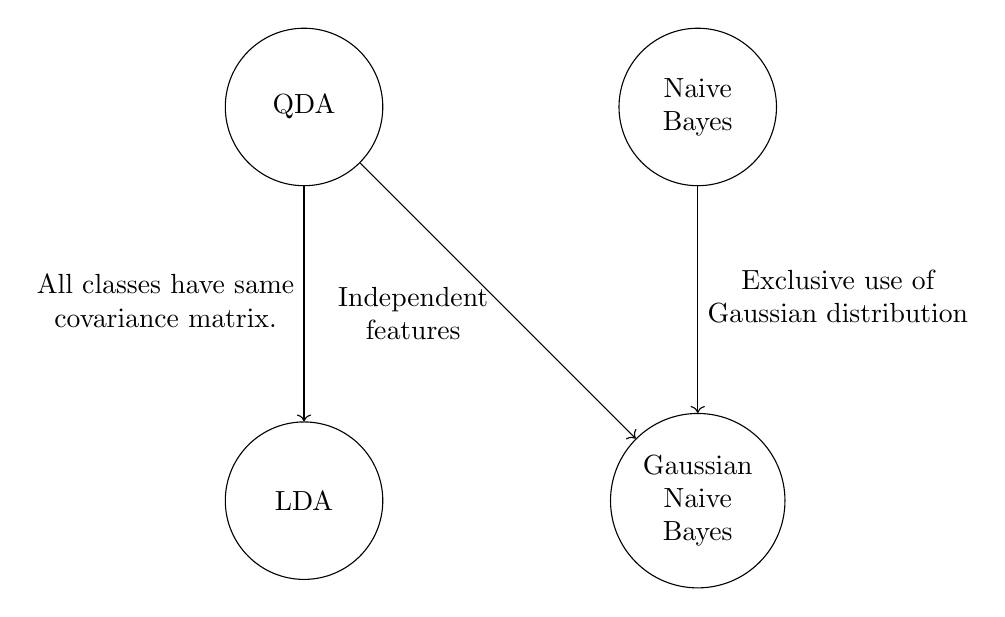
\begin{tikzpicture}[every node/.style={minimum size=2cm}]
        \node[shape=circle,draw=black] (QDA) at (0,0) {QDA};
        \node[shape=circle,draw=black] (NB) at (5,0) {\makecell[c]{Naive\\Bayes}};
        \node[shape=circle,draw=black] (LDA) at (0,-5) {LDA};
        \node[shape=circle,draw=black] (GNB) at (5,-5) {\makecell[c]{Gaussian\\Naive\\Bayes}};

        \path [->] (QDA) edge node[left] {\makecell[c]{All classes have same\\covariance matrix.}} (LDA);
        \path [->] (QDA) edge node[left,yshift=-0.2cm] {\makecell[c]{Independent\\features}} (GNB);
        \path [->] (NB)  edge node[right] {\makecell[c]{Exclusive use of\\Gaussian distribution}} (GNB);
    \end{tikzpicture}
    \caption{ The relationships between all four types of probabilistic classifiers mentioned up until now. }
\end{figure}



\newpage
\begin{appendices}
\section{Derivation of Decision Boudaries for Quadratic Discriminant Analysis}
\begingroup
\allowdisplaybreaks
\begin{align}
    \frac{
        \mathcal{N}(\mu_0, \Sigma_0)  p(y_0) 
    }{
        \mathcal{N}(\mu_1, \Sigma_1)  p(y_1) 
    } &\equnk 1
    \\
    \frac{
        \frac{1}{
        (2\pi)^{\nicefrac{D}{2}} |\Sigma_0|^{\nicefrac{1}{2}}} 
        \exp\left(
            -\frac{1}{2}(x - \mu_0)^T\Sigma_0^{-1}(x-\mu_0)
        \right) p(y_0) 
    }{
        \frac{1}{
        (2\pi)^{\nicefrac{D}{2}} |\Sigma_1|^{\nicefrac{1}{2}}} 
        \exp\left(
            -\frac{1}{2}(x - \mu_1)^T\Sigma_1^{-1}(x-\mu_1)
        \right) p(y_1)
    }
    &\equnk 1
    \\
        \left[ 
            \log{\left(
                \frac{1}{
                    (2\pi)^{\nicefrac{D}{2}} |\Sigma_0|^{\nicefrac{1}{2}}} 
            \right)}
            -\frac{1}{2}(x - \mu_0)^T\Sigma_0^{-1}(x-\mu_0)
            + \log{\left(p(y_0)  \right)}
        \right] \\ \nonumber - \left[
            \log{\left(
                \frac{1}{
                    (2\pi)^{\nicefrac{D}{2}} |\Sigma_1|^{\nicefrac{1}{2}}} 
            \right)}
            -\frac{1}{2}(x - \mu_1)^T\Sigma_1^{-1}(x-\mu_1)
            + \log{\left( p(y_1) \right)}
        \right]
    &\equnk 0
    \\
        \left[ 
            -\frac{1}{2}\log{\left(
                 |\Sigma_0| 
            \right)}
            -\frac{1}{2}(x - \mu_0)^T\Sigma_0^{-1}(x-\mu_0)
            + \log{\left(p(y_0)  \right)}
        \right] \\ \nonumber - \left[
            -\frac{1}{2}\log{\left(
                |\Sigma_1|
            \right)}
            -\frac{1}{2}(x - \mu_1)^T\Sigma_1^{-1}(x-\mu_1)
            + \log{\left( p(y_1) \right)}
        \right]
    &\equnk 0
    \\
        \left[ 
            -(x - \mu_0)^T\Sigma_0^{-1}(x-\mu_0)
        \right]  - \left[
            -(x - \mu_1)^T\Sigma_1^{-1}(x-\mu_1)
        \right]
    &\equnk c
    \\
        -\left[ 
            x^T\Sigma_0^{-1}x
            - 2\mu_0^T\Sigma_0^{-1}x
            + \mu_0^T\Sigma_0^{-1}\mu_0
        \right]  + \left[
            x^T\Sigma_1^{-1}x
            - 2\mu_1^T\Sigma_1^{-1}x
            + \mu_1^T\Sigma_1^{-1}\mu_1
        \right]
    &\equnk c
    \\
        \label{eq:reduce_linear}
        \underbrace{
            x^T \left(
            -\Sigma_0^{-1} + \Sigma_1^{-1}
        \right) x }_{\text{quadratic term}}
        + 
        \underbrace{
        2\left(\mu_0^T\Sigma_0^{-1} - \mu_1^T\Sigma_1^{-1}\right)x}_{\text{linear term}}
        -\underbrace{
         \mu_0^T\Sigma_0^{-1}\mu_0
    + \mu_1^T\Sigma_1^{-1}\mu_1 - c}_{\text{constant term}}
    &\equnk 0
\end{align}
\endgroup

\end{appendices}

\end{document}
